% -*-coding: utf-8 -*-
% Держать в начале каждого файла!

\documentclass[a4paper, 12pt]{extarticle}
\usepackage{metod}

\MTDSetPhysSection{Механика}
\MTDSetTitle{Изучение динамики равномерного движения тела по окружности}
\MTDDesignator{М--7}
\MTDSetGrade{10}

\MTDSetAuthors{И.~Н.~Грачева, В.~И.~Гребенкин, А.~Е.~Иванов, И.~А.~Коротова,
Е.~И.~Красавина, А.~В.~Кравцов, Н.~С.~Кулеба, Б.~В.~Падалкин,
Г.~Ю.~Шевцова, Т.~С.~Цвецинская}

\MTDSetEditorsGenCase{И.~Н.~Грачевой, А.~Е.~Иванова, А.~В.~Кравцова}

\newcommand{\eps}{\epsilon}

\begin{document}

\MTDTitlePage
\MTDInfoPage

\setcounter{section}{7}

\subsection{Цель работы}
Целью работы является экспериментальное исследование законов динамики  материальной точки при ее движении по окружности.

\subsection{Основные теоретические сведения}
При равномерном движении материальной точки по окружности вектор ее скорости, оставаясь по модулю постоянным, изменяет свое направление,  что обусловливает наличие у нее ускорения. В любой точке окружности ускорение направлено к центру (по нормали к траектории) и называется нормальным (центростремительным) ускорением. Модуль нормального ускорения~$a_n$ определяется выражением
\begin{equation}
\label{eq:m7-radial-acc-1}
a_n = \frac{v^2}{r},
\end{equation}
где $v$ "--- модуль линейной скорости материальной точки; $r$ "--- радиус окружности.
% Тут была новая строка и я её убрал, у нас же везде просто в строчку эти вещи после "где"

С учетом известных соотношений
\begin{equation}
\label{eq:m7-angular-velocity}
v = \omega r \quad \text{и} \quad \omega = \frac{2\pi}{T} %нужна ли здесь запятая? | По-моему, нет
\end{equation}
численное значение нормального ускорения может быть выражено через период~$T$: % Поставил по-моему недостававшее двоеточие
\begin{equation}
\label{eq:m7-radial-acc-2}
a_n = \frac{4\pi^2}{T^2}r.
\end{equation}

\subsection{Методика выполнения работы}
Изучение динамики равномерного движения материальной точки по окружности можно выполнить с помощью конического маятника, который представляет собой шарик, подвешенный на нити и равномерно движущийся по окружности (рис.~\ref{fig:m7-conical-pendulum}).

\begin{figure}[h] %немного изменено расположение картинки
\begin{center}
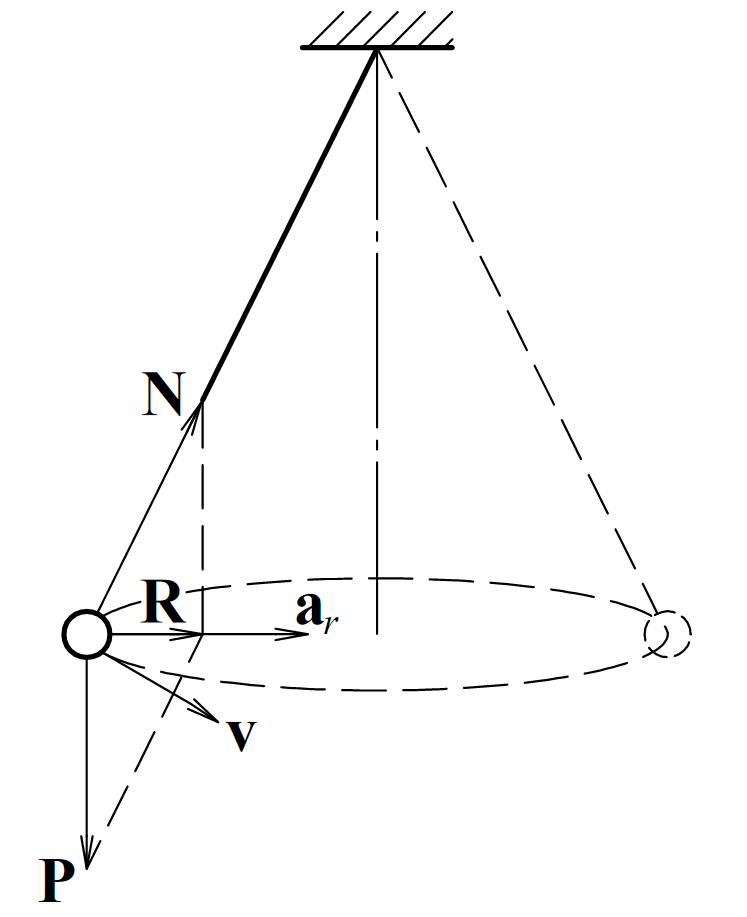
\includegraphics[width=0.3\linewidth, keepaspectratio=true]{M7-ConicPendledumForces}
\end{center}
\caption{Силы, действующие на конический маятник \label{fig:m7-conical-pendulum}}
\end{figure}

На шарик массой~$m$ действуют две силы "--- сила тяжести~$m\vec{g} = \vec{P}$ и сила~$\vec{N}$ натяжения нити. Для любого положения шарика равнодействующая этих сил~$m\vec{a} = \vec{P} + \vec{N}$ направлена к центру окружности и обеспечивает движение шарика с нормальным ускорением~\vec{a}.

В соответствии со вторым законом Ньютона, %нужна ли здесь запятая? | Да
\begin{equation}
\label{eq:m7-2nd-newton's-law}
m\vec{a} = \vec{P} + \vec{N}.
\end{equation}

Модуль равнодействующей определяется выражением
\begin{equation}
\label{eq:m7-resultant-force-1}
R = \sqrt{N^2 - P^2}.
\end{equation}

Учитывая выражение~\eqref{eq:m7-radial-acc-2},
\begin{equation}
\label{eq:m7-resultant-force-2}
R = m\frac{4\pi^2}{T^2}r.
\end{equation}

В работе проводится проверка второго закона Ньютона применительно к равномерному движению материальной точки по окружности. При этом используется методика сравнения значений равнодействующей~$\vec{R}$, вычисленных с помощью выражений~\eqref{eq:m7-resultant-force-1}~и~\eqref{eq:m7-resultant-force-2}.

\subsection{Описание экспериментальной установки}
Схематическое изображение  экспериментальной установки приведено на рис.~\ref{fig:m7-equipment}.

\begin{figure}[h] %немного изменено расположение картинки
\begin{center}
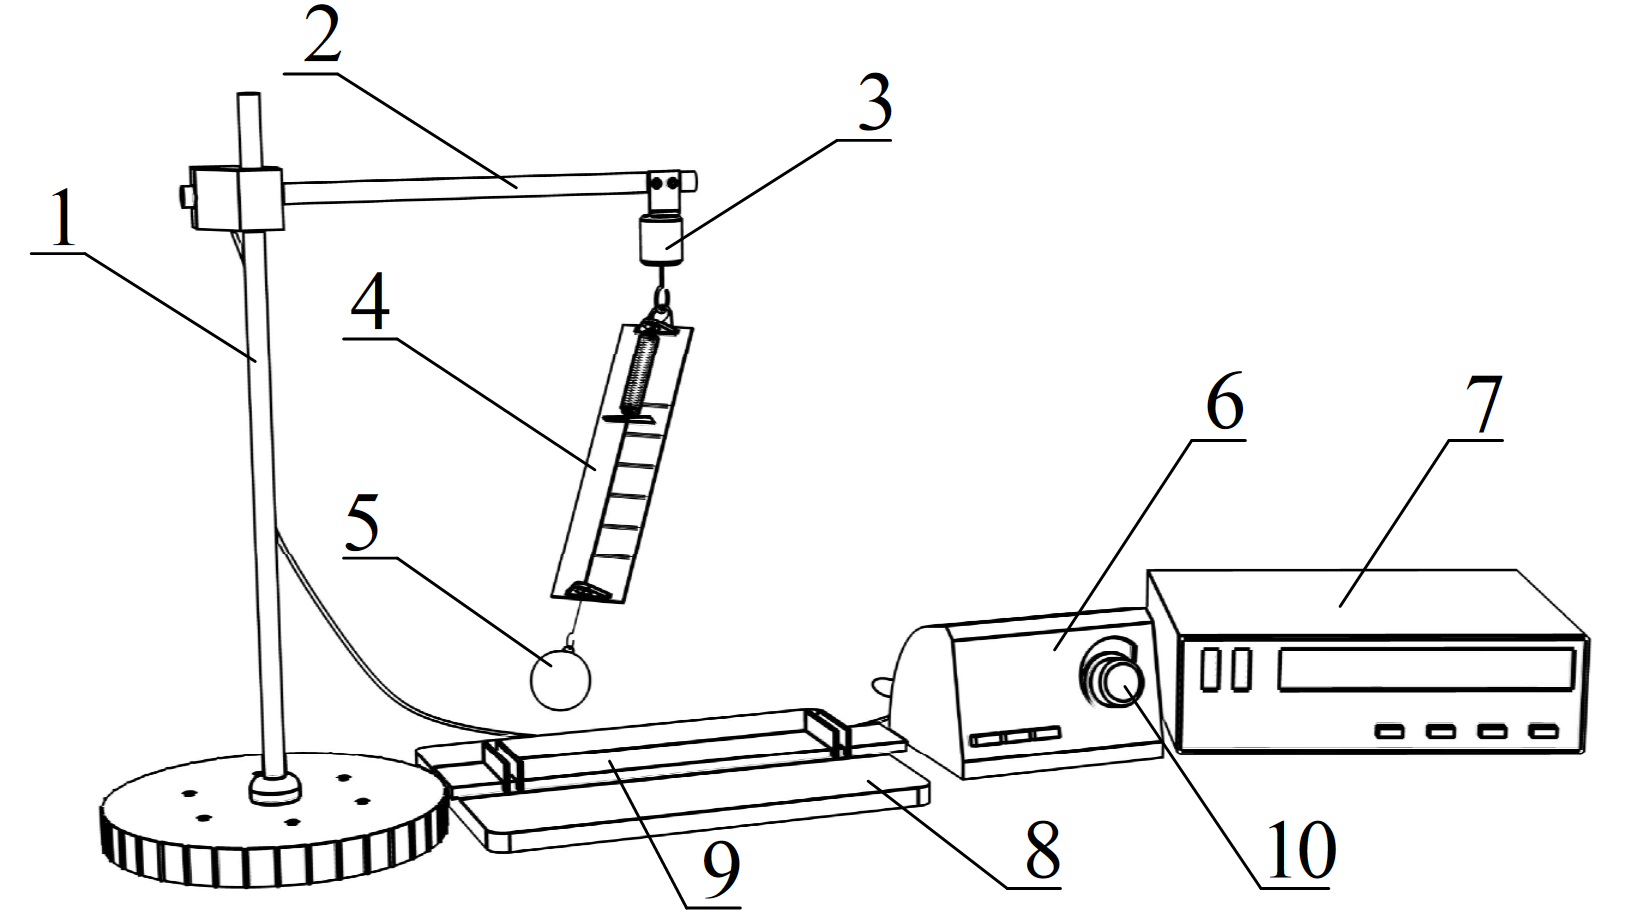
\includegraphics[width=0.6\linewidth, keepaspectratio=true]{M7-BallRotatorMachine}
\end{center}
\caption{Схема экспериментальной установки \label{fig:m7-equipment}}
\end{figure}

Установка состоит из массивной стойки~\emph{1}, с которой связан кронштейн~\emph{2}. К кронштейну прикреплен электродвигатель~\emph{3}, к валу которого прикреплен динамометр~\emph{4} с шариком~\emph{5}. Электродвигатель питается от источника~\emph{6}. Угловая скорость вращения вала регулируется ручкой~\emph{10} регулятора напряжения. Подаваемое на электродвигатель напряжение измеряется вольтметром~\emph{7}. Для измерения радиуса окружности, по которой движется шарик, используется планшет~\emph{8} с линейкой~\emph{9}, которые располагаются под динамометром с шариком. Динамометр снабжен муфтой, свободно перемещающейся  вдоль шкалы и обеспечивающей снятие показания динамометра после остановки системы: указатель пружины, надавливая на муфту, смещает ее. С помощью динамометра также производится взвешивание шариков.

\subsection{Порядок выполнения работы}
\begin{enumerate}
\item Значение массы шарика и приборную погрешность запишите в таблицу~\ref{tab:m7-res-exp}.

\begin{table}[H]
\caption{\label{tab:m7-res-exp}} \vspace{-10pt} % Чуть приблизил название к таблице
\begin{flushright}
\begin{tabular}{|>{\centering\arraybackslash} m{2.6cm}|>{\centering\arraybackslash} m{0.995cm}|>{\centering\arraybackslash} m{0.995cm}|>{\centering\arraybackslash} m{0.995cm}|>{\centering\arraybackslash} m{0.995cm}|>{\centering\arraybackslash} m{0.995cm}|>{\centering\arraybackslash} m{0.995cm}|>{\centering\arraybackslash} m{0.995cm}|>{\centering\arraybackslash} m{0.995cm}|>{\centering\arraybackslash} m{0.995cm}|}
\hline
\multirow{2}{2.6cm}{\centering Измеряемые величины} & \multirow{2}*{$m,~\text{\Units{кг}}$} & \multirow{2}*{$P,~\text{\Units{Н}}$} & \multirow{2}*{$r,~\text{\Units{м}}$} &  \multicolumn{3}{c|}{$t,~\text{\Units{c}}$} & \multirow{2}*{\hspace{3pt}$\MTDMean{t},~\text{\Units{с}}$} & \multirow{2}*{$T,~\text{\Units{с}}$} & \multirow{2}*{$N,~\text{\Units{Н}}$} \\ \cline{5-7}
      & & & & 1 & 2 & 3 & & & \\ \hline
	Значение & & & & & & & & & \\ \hline
       Погрешность & & & & & & & & & \\
       \specialrule{.15em}{0em}{0em} % Поставил жирную линию
Расчетные величины & \multicolumn{3}{c|}{$a_n,~\Units{\text{м}/\text{с}^2}$} & \multicolumn{3}{c|}{$ma_n,~\Units{\text{Н}}$} & \multicolumn{3}{c|}{$R,~\Units{\text{Н}}$} \\ \hline
      Значение & \multicolumn{3}{c|}{} & \multicolumn{3}{c|}{} & \multicolumn{3}{c|}{} \\ \hline
      Погрешность & \multicolumn{3}{c|}{} & \multicolumn{3}{c|}{} & \multicolumn{3}{c|}{} \\ \hline
\end{tabular}
\end{flushright}
\end{table}

\item Наденьте динамометр с подвешенным шариком на крючок вала электродвигателя так, чтобы шарик немного не касался плоскости планшета. Придвиньте муфту вплотную к указателю.
\item Включите источник~\emph{6}, при этом должна загореться сигнальная лампа.  Вращением ручки~\emph{10} подайте на электродвигатель напряжение, указанное на приборе (около 40~\Units{В}), измеряя его вольтметром~\emph{7}. При этом вал электродвигателя начнет вращение, вовлекая в движение подвешенный динамометр с шариком.
\item Выждите 5--10~минут, пока режим вращения не установится. Установление режима можно определить, поместив визир линейки под одно из крайних положений шарика и убедившись, что центр шарика будет все время проходить над визиром. После этого под другое крайнее положение шарика поставьте второй визир, зафиксировав тем самым диаметр окружности вращения шарика.
\item Измерьте три раза с помощью секундомера время $t$ десяти ($n = 10$) оборотов маятника. Данные запишите в таблицу~\ref{tab:m7-res-exp}.
\item Вращением ручки~\emph{10} регулятора напряжения остановите вращение установки. По положению муфты динамометра определите силу~$T$, с которой была натянута пружина динамометра при равномерном вращении маятника.
\item По расстоянию между визирами вычислите радиус вращения шарика.
\item Пользуясь разделом~В.4, определите погрешности прямых измерений, проведите расчеты по выражениям~\eqref{eq:m7-2nd-newton's-law}~и~\eqref{eq:m7-resultant-force-1}, заполните таблицу~\ref{tab:m7-res-exp}.
\item Напишите заключение к работе.

\textbf{Расчетные соотношения}: %мб все формулы выносные | Да, у нас всё равно меньше 6 страниц не получится, ИЗМ: сделал жирным и сделал выносные формулы, оказалось, они даже на следующую страницу не залезают
\begin{align*}
&m,\ P,\ r,\ N,\ t\ \text{"--- данные прямых измерений,} \\
&\Delta m,\ \Delta P,\ \Delta r,\ \Delta N\ \text{"--- приборные погрешности,} %а \Delta t? | Выглядит, как будто пропустили, добавил | не, там не надо, потому что там другая погрешность будет за счет нескольких измерений
\end{align*} \begin{align*} 
\Delta (ma) &= ma\sqrt{\eps_r^2 + (2\eps_T)^2}, \\ %убрала скобки вокруг ma, зачем они?
\Delta T &= \dfrac{\Delta t}{n}, \\
T &= \dfrac{\MTDMean{t}}{n}, \\
\Delta R &\approx \Delta N \left(\dfrac{R}{P}\right)^2.
\end{align*}
\end{enumerate}

\subsection{Контрольные вопросы}
\begin{enumerate}
\item Для нормального ускорения известны два выражения: $a_n = v^2\kern-.15em/r$ и $a_n = \omega^2 r$. Усматриваете ли Вы противоречие в том, что, согласно одному из них, ускорение обратно пропорционально, а, согласно другому, "--- прямо пропорционально радиусу $r$ окружности, по которой движется материальная точка? %\dfrac - некрасиво ИЗМ: вопрос в конце предложения | Поменял dfrac на обычную косую черту
\item Можно ли утверждать, что равномерное движение материальной точки по окружности происходит под действием постоянной силы? С постоянным ускорением? Почему?
\end{enumerate}

\end{document}
